\documentclass[a4paper,10pt,oneside]{article}
\usepackage[polutonikogreek,italian]{babel}
\usepackage[utf8x]{inputenc}
\usepackage{amsmath}
\usepackage{amsthm}
\usepackage{amssymb}
\usepackage{amscd}
\usepackage{graphicx}
\usepackage{float}
\usepackage{array}
\usepackage{rotating}
\usepackage[small]{caption}
\usepackage{lscape}
\usepackage{fancybox}
\usepackage{booktabs}
\usepackage[noanswer]{exercise}
\parindent0ex
\renewcommand{\fboxsep}{0.4cm}
\usepackage{hyperref}
\renewcommand{\textfraction}{0.05}
\renewcommand{\topfraction}{0.95}
\renewcommand{\bottomfraction}{0.95}
\renewcommand{\floatpagefraction}{0.35}
\renewcommand{\ExerciseName}{Esercizio}
\renewcommand{\ExerciseListName}{Es}
\setcounter{totalnumber}{5}
\restylefloat{figure}
\begin{document}
 \section*{Potenza e Lavoro}
Durante la lezione abbiamo definito la potenza media come il rapporto tra il lavoro ed il tempo in cui questo lavoro viene speso:
\begin{equation}\label{p_media}
 P=\frac{L}{T}
\end{equation}
partendo dalla definizione di potenza media possiamo definire anche una potenza istantanea:
\begin{equation}
 P=\frac{F\Delta S}{\Delta T}
\end{equation}
riducendo via via l'intervallo temporale $\Delta T$ il rapporto $\Delta S /\Delta T$ si avvicinerà sempre più alla velocità istantanea del corpo all'istante $T$
da cui
\begin{equation}
 P(t)=Fv(t)
\end{equation}
Studiamo ora due casi particolari nei quali potremo definire una potenza istantanea, ovvero la velocità con cui viene speso il lavoro in un determinato tempo.
\subsection*{Forza costante e velocità costante}
Immaginiamo che il corpo cui è applicata la forza $F$, costante, si muova a velocità costante $v$, il lavoro speso dalla forza al tempo $T$ sarà quindi:
\begin{equation}
 L=FS(T)=FvT
\end{equation}
dove $vT$ è lo spazio percorso nel tempo $T$.
La potenza media risulterà quindi:
\begin{equation}\label{p_ist}
 P=\frac{L}{T}=Fv
\end{equation}
la potenza istantanea è in questo caso identica alla potenza media dato che la velocità è costante e quindi  tratti spaziali uguali vengono percorsi in tempi uguali
\begin{figure}[H]
 \centering
 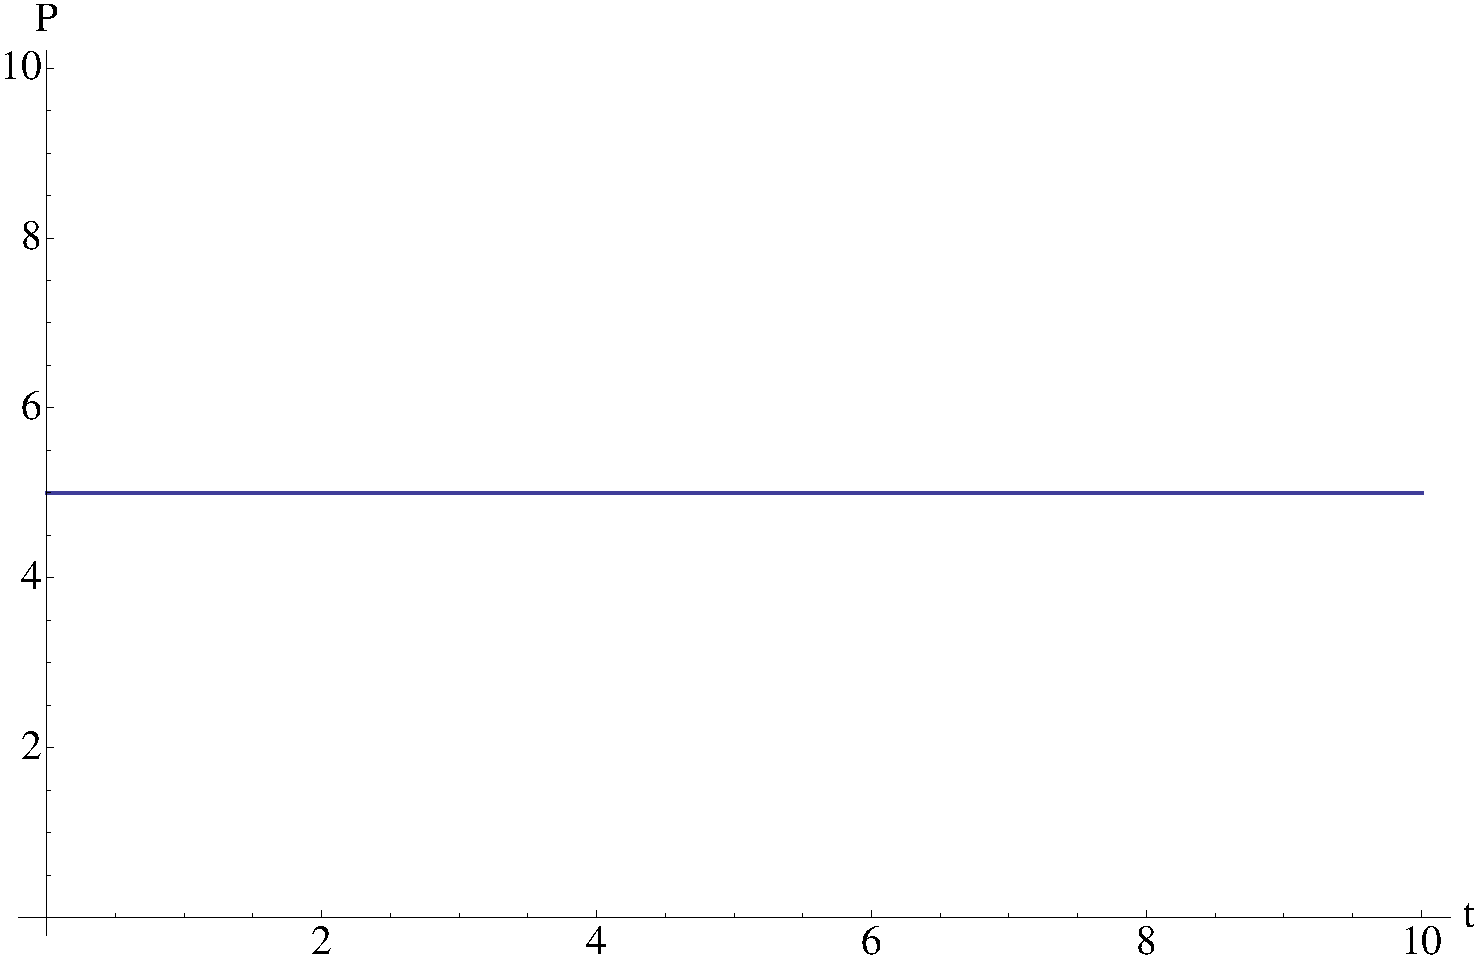
\includegraphics[width=0.8\textwidth]{./immagini/potenza_costante.pdf}
 % potenza_costante.pdf: 708x462 pixel, 72dpi, 24.98x16.30 cm, bb=0 0 708 462
 \label{fig:potenza_costante}
\end{figure}
Notiamo come se il corpo si muove a velocità costante, nonostante gli sia applicata la forza $F$, si debba  supporre l'azione di almeno un'altra forza poiché  in un sistema inerziale il primo principio della dinamica ci dice che se un corpo si muove di moto rettilineo uniforme allora la forza \textbf{totale} ad esso applicata è nulla.
Una applicazione estremamente utile del concetto di potenza si ha nel calcolo del lavoro eseguito da una forza data la potenza istantanea e il tempo per cui la forza viene applicata.
Nel caso in esame la potenza istantanea è uguale alla potenza media per cui possiamo dire che il lavoro eseguito risulterà essere:
\begin{equation}
 L=PT
\end{equation}
risultato che possiamo leggere nel grafico [\ref{fig:potenza_lavoro1}] come l'area sottesa dalla curva $P(t)$.

\begin{figure}[H]
 \centering
 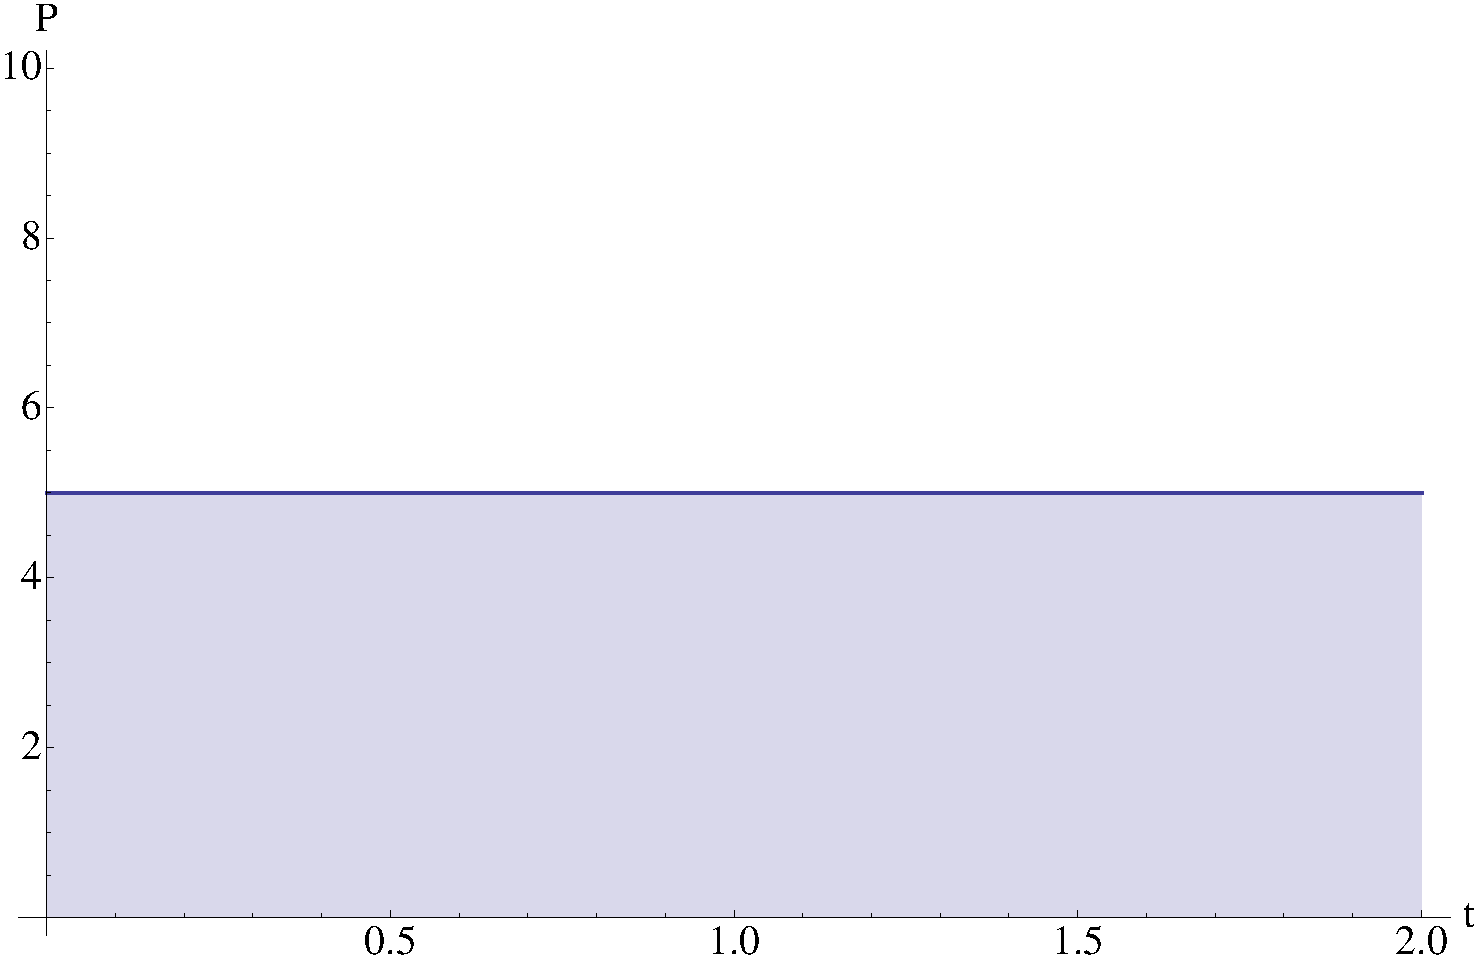
\includegraphics[width=0.8\textwidth]{./immagini/potenza_costante_lavoro.pdf}
 % potenza_costante_lavoro.pdf: 708x462 pixel, 72dpi, 24.98x16.30 cm, bb=0 0 708 462
 \caption{Il lavoro eseguito dalla forza è pari all'area sottosa dalla curva $P(t)$}
 \label{fig:potenza_lavoro1}
\end{figure}


\subsection*{Forza costante e velocità non costante}

Supponiamo ora che un corpo di massa $M$, inizialmente fermo, stia accelerando con accelerazione costante $a$ data dalla forza costante $F$ ad asso applicata (se questa è l'unica forza agente) o dalla somma delle forze applicate al corpo.
La costanza dell'accelerazione ci permette di calcolare semplicemente  il valore della velocità del corpo in ogni istante di tempo:
\begin{equation}
 v(t)=at
\end{equation}
e parimenti lo spazio percorso dal corpo al tempo $T$:
\begin{equation}
 S(T)=\frac1 2 aT^2
\end{equation}

il lavoro svolto al tempo $T$ sarà quindi:
\begin{equation}
 L(T)=FS(T)=F\frac{1}{2}aT^2
\end{equation}
la potenza media:
\begin{equation}
 P=\frac{F\frac{1}{2}aT^2}{T}=F\frac 1 2 aT
\end{equation}

la potenza istantanea sarà in questo caso diversa dalla potenza media dato che il corpo percorre spazi diversi in tempi uguali. Applicando però la [\ref{p_ist}] e la definizione di velocità nel moto uniformemente accelerato possiamo scrivere:
\begin{equation}
 P(t)=Fv(t)=Fat
\end{equation}
vediamo quindi che la potenza dissipata dalla forza $F$ aumenta linearmente con il tempo
\begin{figure}[H]
 \centering
 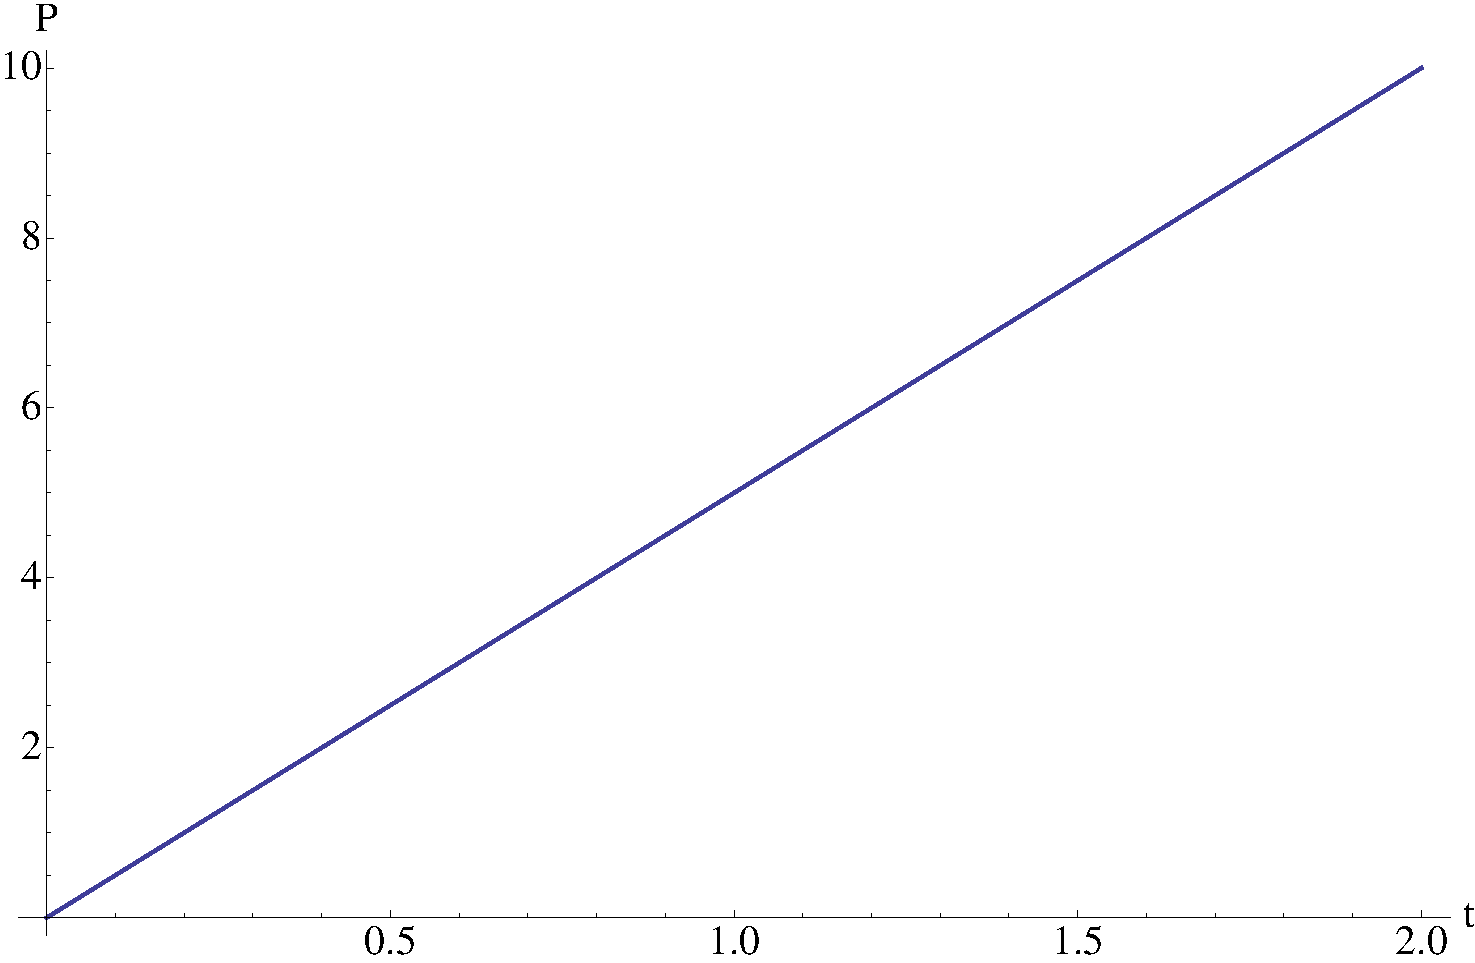
\includegraphics[width=0.8\textwidth]{./immagini/potenza_lineare.pdf}
 % potenza_lineare.pdf: 708x462 pixel, 72dpi, 24.98x16.30 cm, bb=
 \label{fig:potenza_lineare}
\end{figure}
Il calcolo del lavoro a partire dalla potenza e dal tempo di applicazione della forza può essere ripetuto anche nel caso in cui la potenza non sia più costante.

\begin{figure}[H]
 \centering
 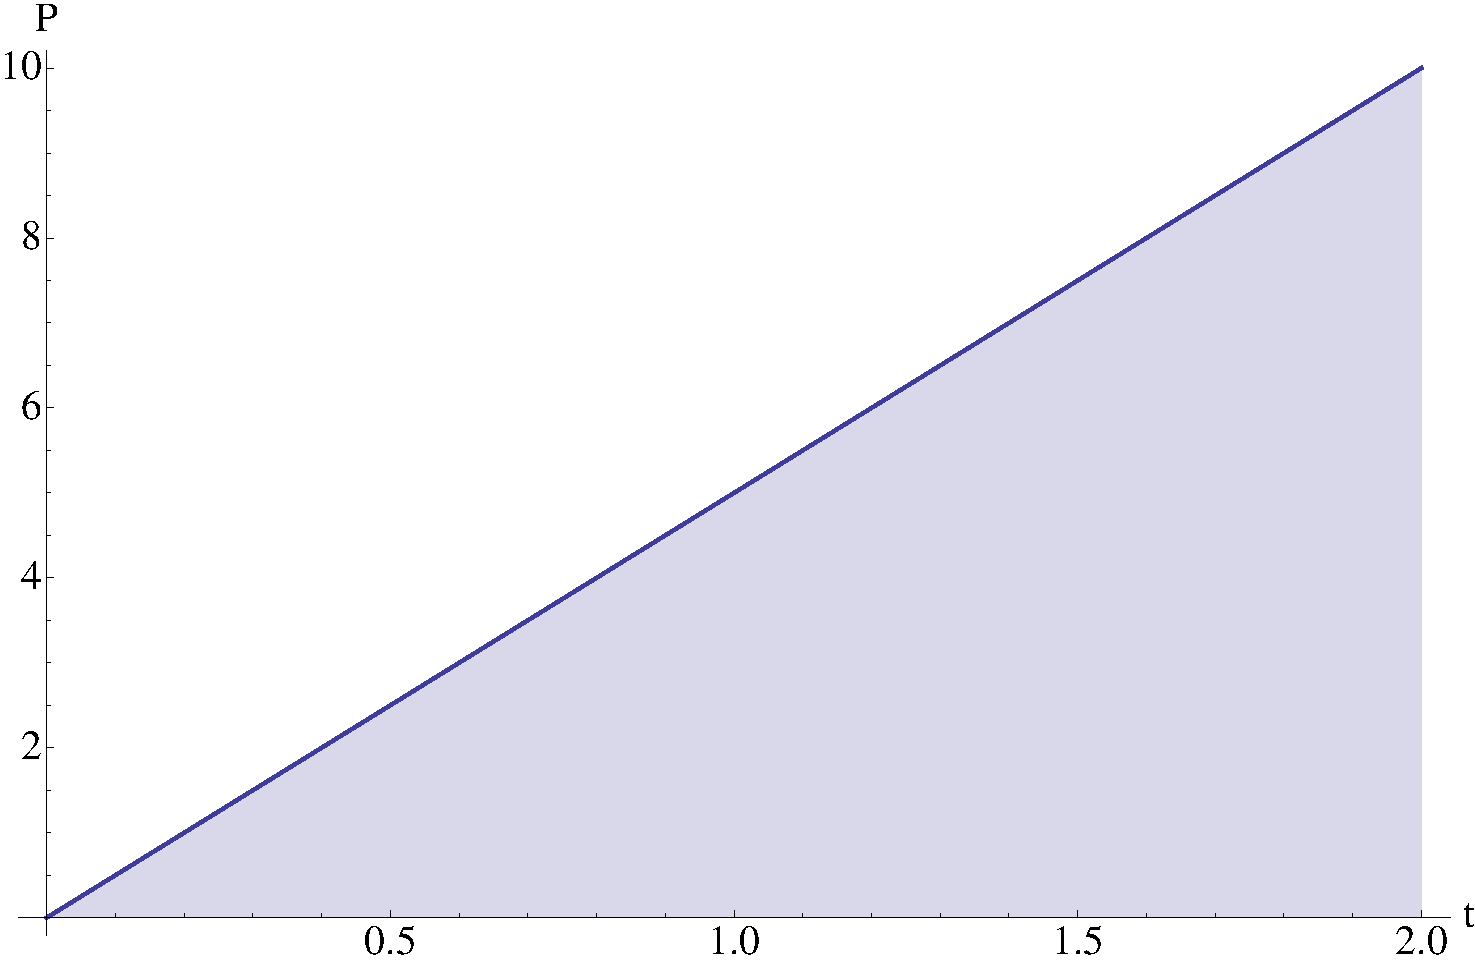
\includegraphics[width=0.8\textwidth]{./immagini/potenza_lavoro2.pdf}
 % potenza_lavoro2.pdf: 708x462 pixel, 72dpi, 24.98x16.30 cm, bb=0 0 708 462
 \caption{Nel caso in cui la relazione potenza tempo è lineare il lavoro è rappresentato dall'area del triangolo sotteso dalla curva $P(t)$}
 \label{fig:pot_lav2}
\end{figure}


Per giustificare l'interpretazione del lavoro compiuto come l'area sottesa dalla curva $P(t)$ immaginiamo di suddividere il triangolo di figura [\ref{fig:pot_lav2}] in tanti rettangoli, in ognuno di questi rettangoli immaginiamo che la potenza sia costante, il lavoro speso in ognuno di questi rettangoli sarà quindi pari al caso visto precedentemente, il lavoro totale generato durante tutto l'arco temporale si otterrà sommando i valori delle aree di tutti i rettangoli, si può dimostrare che al tendere a zero dell'ampiezza della base dei rettangoli il valore dell'area diventa pari all'area del triangolo:
\begin{equation}\label{pot_var}
 L=\frac 1 2 FaT^2
\end{equation}

il risultato espresso nella [\ref{pot_var}] è proprio ciò che ci aspettiamo dato che $\frac 1 2 aT^2$ è il tratto percorso dall'oggetto nel tempo $T$.

\subsection*{Un breve esercizio}

Immaginiamo di avere a disposizione una macchina di massa $m$ con carburante sufficiente ad erogare un lavoro pari a $L$. Dobbiamo percorrere una distanza $l$ consumando tutto il carburante disponibile, la macchina è dotata di un motore in grado di produrre potenze arbitrariamente grandi, l'unica forza che considereremo presente nel sistema sarà quella motrice costante del propulsore. Che strategia dobbiamo utilizzare per minimizzare il tempo necessario a coprire il tratto $l$
?
Per prima cosa notiamo che la massima velocità raggiungibile consumando tutto il carburante è pari a:
\begin{equation}\label{vel_max}
 v_f=\sqrt{\frac{2L}{m}}
\end{equation}
Il risultato [\ref{vel_max}] è stato ottenuto utilizzando la relazione tra energia cinetica e lavoro\footnote{Anche noto come teorema dell'energia cinetica $L=\frac 1 2 mv_f^2-\frac 1 2 mv_i^2$}.

Analizziamo per primo il caso  in cui il carburante finisce esattamente alla fine del tragitto, la forza motrice della macchina risulta:
\begin{equation}
 F=\frac{L}{l}
\end{equation}
l'accelerazione costante cui è sottoposta la macchina:
\begin{equation}
 a=\frac F m =\frac{L}{ml}
\end{equation}
il tempo necessario per percorrere la distanza $l$ diventa quindi:
\begin{equation}
 t_1=\sqrt{\frac{2l^2m}{L}}=l\sqrt{\frac{2m}{L}}
\end{equation}
Notiamo che in questo primo caso la velocità massima è assunta dalla macchina al termine del tragitto.

Il secondo caso che è utile trattare è quello in cui il motore eroga una potenza infinita per un tempo infinitesimo in questa situazione estrema possiamo ammettere che il lavoro $L$ venga speso lungo una distanza spaziale nulla, per tanto la macchina si muove con velocità pari alla velocità massima sin dal primo istante. Come abbiamo già calcolato tale velocità risulta essere data dalla [\ref{vel_max}] il tempo di percorrenza diventa allora:
\begin{equation}
 t_2=\frac{l}{v_f}=l\sqrt{\frac{m}{2L}}
\end{equation}
confrontiamo ora i due tempi $t_1$ e $t_2$:
\begin{equation}
 \frac{t_1}{t_2}=l\sqrt{\frac{2m}{L}}\frac{1}{l}\sqrt{\frac{2L}{m}}=2
\end{equation}
vediamo quindi che nel caso in cui la nostra macchina fosse in grado di fornire una potenza infinita il tempo minimo di percorrenza sarebbe pari alla metà del tempo massimo.


\end{document}
